% Класс документов по ГОСТ 7.32-2001 "Отчёт о научно-исследовательской работе"
% на основе ГОСТ 2.105-95
% Автор - Алексей Томин, с помощью списка рассылки latex-gost-request@ice.ru,
%  "extreport.cls", "lastpage.sty" и конференции RU.TEX
% Лицензия GPL
% Все вопросы, замечания и пожелания сюда: mailto:alxt@yandex.ru
% Дальнейшая разработка и поддержка - Михаил Конник,
% связаться можно по адресу mydebianblog@gmail.com

\documentclass[utf8,usehyperref,12pt]{G7-32}
\usepackage[T2A]{fontenc}
\usepackage[utf8]{inputenc} %% ваша любимая кодировка здесь
\usepackage[english,russian]{babel} %% это необходимо для включения переносов
\usepackage{float}
\usepackage{graphicx}
\graphicspath{{pictures/}}

\TableInChaper % таблицы будут нумероваться в пределах раздела
\PicInChaper   % рисунки будут нумероваться в пределах раздела
\setlength\GostItemGap{2mm}% для красоты можно менять от 0мм

% Определяем заголовки для титульной страницы
\NirOrgLongName{\textsc{НАЦИОНАЛЬНЫЙ ИССЛЕДОВАТЕЛЬСКИЙ ЯДЕРНЫЙ УНИВЕРСИТЕТ «МИФИ» }} %% Полное название организации

\NirBoss{Директор ООО <<Рога и Копыта>>}{И.И.Иванов} %% Заказчик, утверждающий НИР
\NirManager{инженер}{Д.Е. Катаев} %% Название организации

\NirYear{2013}%% если нужно помен\label{?} ять год отчёта; если закомментировано, ставится текущий год
\NirTown{г. Москва,} %% город, в котором написан отчёт
% по проекту \No8550: 

% \NirIsAnnotacion{АННОТАЦИОННЫЙ } %% Раскомментируйте, если это аннотационный отчёт

\NirUdk{УДК \No 2123132123}
\NirGosNo{Регистрационный \No 123123}

\NirStage{Этап \No 1.1}{промежуточный}{<<Обзор современного состояния торсионных наногенераторов>>} %%% Этап НИР: {номер этапа}{вид отчёта - промежуточный или заключительный}{название этапа}

\bibliographystyle{unsrt} %Стиль библиографических ссылок БибТеХа

%%%%%%%<------------- НАЧАЛО ДОКУМЕНТА
\begin{document}
\usefont{T2A}{ftm}{m}{} %%% Использование шрифтов Т2 для возможности скопировать текст из PDF-файлов.

\frontmatter %%% <-- это выключает нумерацию ВСЕГО; здесь начинаются ненумерованные главы типа Исполнители, Обозначения и прочее

\NirTitle{\textbf{«Оптимизация обучающих выборок с помощью генетического алгоритма»}} %%% Название НИР и генерация титульного листа«»


\Executors %% Список исполнителей здесь
%% это рисует линию размера 3мм и толщиной 0.1 пункт
\begin{longtable}{p{0.35\linewidth}p{0.2\linewidth}p{0.35\linewidth}}
Научный руководитель, 	&		&	\\
доцент К.К.Петров	&\rule{1\linewidth}{0.1pt}	&  \\ \vspace{1cm}

с.н.с, к.т.н,  &		&	\\
Ж.Ж. Балбесов, & \rule{1\linewidth}{0.1pt}& \\
\end{longtable}
\Referat
 Отчет \totalpages~с, \totaltables~таблица, \totalfigures~рисунок, \totalbibs~источник.
\tableofcontents

\Introduction
Одним из ключевых моментов в реализации систем, использующих алгоритмы машинного обучения с учителем является подготовка обучающей выборки. В настоящее время, как правило, синтез обучающей выборки выполняется экспертом.ъ, который, однако, далеко не для всех задач в состоянии за разумное время выбрать и представить исходные данные задачи в оптимальном для обучаемой системы виде. Таким образмо имеется потребонсть в системах, которые способны автоматически формировать обучающие выборки для интеллектуальных систем из имеющихся данных таким образом, чтобы их обучение по автоматически сформированным выборкам было максимально эффективным. Естественно, подобные системы востребованы только в тез случаях, когда либо не существует, либо не сформулирован алгоритм формирования обучающей выборки. Таким образом наиболее иодходящим выглядит использование алгоритмов случайного поиска, например генетических.

Цель данной работы разработка новой версии ПО для генетической оптимизации обучющих выборок систем машинного обучения с учителем. Модификация алгоритма для устранения избыточности обучающих данных. А так же оценка класса решаемых алгоритмом задач.

\mainmatter %% это включает нумерацию глав и секций в документе ниже
% Ниже следует неотрефакторенный текст.
\chapter{Постановка задачи}
Основной задачей являлась разработка новой версии программного обеспечения для оптимизации обучающих выборок при помощи генетического алгоритма на основе старой с реализацией ряда модификаций:
\begin{enumerate}
\item Модификация структуры хранения данных
\item Устранение избыточности обучающих данных
\item Модификация алгоритма мутации для реализации рекурсивной мутации
\item Реализация на Python
\end{enumerate}
\section{Описание исходной системы}
Пусть $ f(S_{h})=(S_{t}; S_{v})) $ - отображение $f$ исторических данных $S_{h}$ в совокупность обучающей $S_{t}$ и валидационной $S_{v}$ выборок. Пусть $ N(S_{t}; S_{v}) $ - искусственная нейронная сеть прямого распространения, обученная по $S_{t}$ и проверяемая по $S_{v}$, а $ Err_{v}(N(S_{t}; S_{v})) $ - ее ошибка валидации, определяемая, как среднеквадратичное отклонение всех выходов сети от соответствующих эталонных значений при подаче на вход элементов валидационной выборки. Тогда
\begin{equation}
\exists\bar{f}:\bar{f}(S_{h})=arg\{min Err_{v}(N(S_{t}; S_{v})). \}
\end{equation}
Требуется найти $ \bar{f} $. Для этого реализован следующий алгоритм, представленный на рис. ~\ref{algo} \\
Критерием останова в используемой реализации является прохождение заданного количества итераций. В текущей реализации используются ИНС прямого распространения в одним скрытым слоем, обучаемые методов эластичного распространения (RPROP)\\
Отображения $f$ представляют собой конструкции следующего вида:
\begin{equation}
f(S_{h})=\begin{array}{|c|}
(\lambda_{i_{1}} \circ \lambda_{i_{2}} \circ ... \circ \lambda_{i_{m}})(S_{h_{j_{1}}}) \\
...\\
(\lambda_{i_{n-l}} \circ ... \circ \lambda_{i_{n}})(S_{h_{j_{k}}})
\end{array}
, \lambda\in\Lambda, i,n,m,j\in N,
\end{equation}
где $\Lambda$ - множество доступных системе элементарных преобразований сигналов (дифференцирование, фильтры, добавление лагов и т.п.), $S_{h_{j}}$ - произвольный сигнал из исторических данных. Атомарной единицей при кроссовере является $f(S_{h})_{i}$, однако мутации возможны и внутри нее.\\
\begin{figure}[H]
 \caption{Схема используемого алгоритма}\label{algo}
 \centering{
 	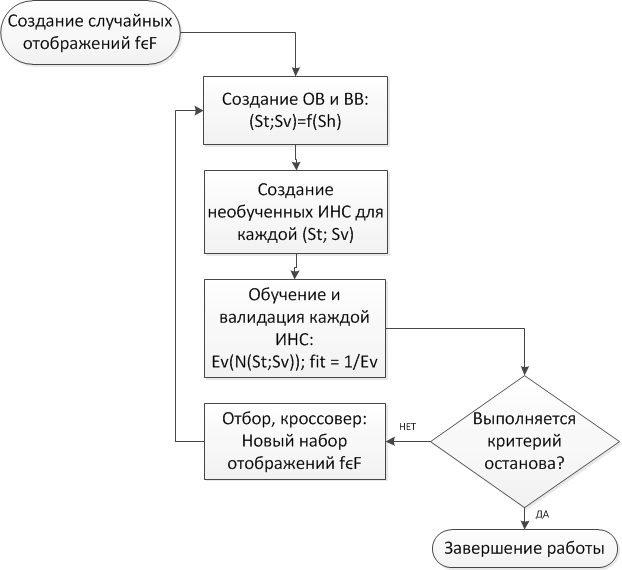
\includegraphics[width=0.4\textwidth]{algo.png}
  }
\end{figure}

При хранении экземпляр кодировался линейной последовательностью исполняемых команд и списком команд, результаты выполенения которых попадают в обучающую выборку. Такая структура данных не способствовала тонкой настройке алгоритмов кроссовера и мутации.
\section{описание стоящих задач}
\subsection{Модификация структуры хранения данных}
В силу тяжести взаимодействия человека с исходным форматом хранения данных было решено сменить формат хранения данных при смене версии приложения. Целями смены формата было повышение читаемости человеком, легкости транспортировки и модифицирования данных эксперимента, но при этом сохранение, по возможности легкости загрузки данных в приложение, для возможности восстановить экземпляры полученные в ходе эксперимента.

Возможными структурами хранения при решении данной задачи были xml, json, исполняемый код или хранение в реляционной базе данных. К плюсам xml при решении поставленной задачи следует отнести следующее:
\begin{enumerate}
\item Возможность прочтения человеком структуры эксперимента в достаточно читаемом виде при наличии достаточно примитивных средств просмотра (Все остальные способы не отличаются простотой)
\item Достаточно легкая транспортабельность результатов эксперимента при необходимости. (Это преимущество работает, пожалуй, только относительно хранения в базе данных)
\end{enumerate}
По результатам выбора между представленными альтернативами был выбран формат данных xml.

\subsection{Устранение избыточности обучающих данных}
В предыдущей версии возникла проблема избыточности размера экземпляров, которая при длительном ходе эксперимента могла достаточно критично повлиять на объем излишних вычислений, производимых системой. Задачей является сокращение роста избыточности экземпляров, при сохранении притом возможности такого роста.

Устранить избыточность обучающих данных можно было при помощи нескольких модификаций:
\begin{enumerate}
\item Выкидывание на каждой мутационной фазе алгоритма одного элемента из экземпляра и проверка направления изменения фитнесс-функции
\item Жесткое ограничение на размер экземпляра
\item Изменения распределения вероятностей в пользу уменьшения, а не увеличения размера экземпляра
\end{enumerate}
Вариант с жестким ограничением на размер экземпляра был отвергнут в связи с предугадать рельную правильную длину. Вариант с изменением алгоритма мутации был исключен в силу увеличения времени работы каждого шага почти в два раза. Реализуемым вариантом стал вариант с изменением распределения вероятностей. Конкретным изменением послужило увеличение возможного интервала размеров на следующем шаге в сторону уменьшения.

\subsection{Модификация алгоритма мутации для реализации рекурсивной мутации}
Для осуществления возможности вносить большее разнообразие в экземпляры и большей настраивамости хода работы алгоритма требовалось введение возможности мутировать не только атомарные объекты но и блоки этих объектов.

Для реализации рекурсивной мутации в каждой сущности, вплоть до атомарного элемента - функции ЦОС, была модифицирована процедура мутации. На фазе мутации каждая сущность верхнего уровня с заданной вероятностью мутировала полностью - генерировался полностью новый экземпляр этой сущности, в обратном же случае она вызывала мутацию всех своих сущностей-детей.

\subsection{Реализация на Python}
В ходе разработки новой версии возникла потребность реализовать систему набором средств предоставляющих инструментарий для легкой поддержки и модификации системы.

В качестве языка разработки был выбран python версии 2.7. python на данный момент является широко распространенным языком для научной разработки. Набор библиотек позволяет не заниматься реализацией большинства общепринятых алгоритмов, например алгоритм обучения с учителем. Язык обладает четким и последовательным синтаксисом, а так же хорошей масштабируемостью, что позволяет сохранить читаемость, сопровождаемость и дополняемость кода. К тому же Python умеет работать с такими языками как Fortran, C и С++, которые уже широко используются в научных расчетах.

\chapter{Описание результата разработки}
\chapter{Эксперименты}
\section{Используемые тестовые сценарии}
Для тестирования использовалось два типа систем - линейная и нелинейная. Под сценарием эксперимента подразумевается набор из входных и целевых данных для нейросети.
\subsection{Линейная система}
Пусть существует бассейн, который является объектом управления. К нему подведены две трубы: через одну в бассейн может поступать вода с произвольной скоростью (в данном тестовом сценарии не будут учитываться физические ограничения), через вторую трубу вода может уходить из бассейна с произвольной скоростью. Через эти две трубы осуществляется управление бассейном. Ограничения на то, что объем воды в бассейне должен быть неотрицательным нет, но, стоит отметить, что в данном сценарии не возникает соответствующей ситуации.\\
Пусть существуют следующие экспериментальные данные:\\
$ X^{(0)} $ – объем поступившей за $ \Delta t $ воды;\\
$ X^{(1)} $ – объем откачанной за $ \Delta t $ воды;\\
$ X^{(2)} $ – объем воды, находящейся в бассейне в данный момент времени;\\
$ X^{(3)} $ – посторонний сигнал, отличающийся от остальных;\\
Реально бассейн реагирует на управляющие воздействия следующим образом:\\
\begin{equation}
X^{(2)}_{i} = X^{(2)}_{i-1} + X^{(0)}_{i-1} - X^{(1)}_{i-1}; X^{(2)}_{0}=10
\end{equation}


Пусть испытуемая система не имеет априорной информации об объекте управления и имеет доступ к следующим данным в качестве исходных:\\
$ X^{(0) \Delta t} $ – объем поступившей за $ \Delta t $ воды, на этот сигнал наложен импульсный шум (inflow\_noizd);\\
$ X^{(1) \Delta t} $ – объем откачанной за $ \Delta t $ воды (outflow);\\
$ X^{(3)} $ – посторонний сигнал (trash).\\
Главной целью системы является верно спрогнозировать динамику изменения уровня воды в бассейне, то есть $ \frac{dX^{(2)}}{dt} $ .
\subsection{Нелинейная система}


\section{Устранение избыточности}
В качестве эксперимента для проверки работоспособности решения по устранению избыточности было решено провести пару тестов на одинаковых входных данных для старого и нового алгоритмов кроссовера. В качестве метрики для сравнения был выбран размер экземпляра на определенной итерации, усредненный среди нескольких экспериментов, для устранения возможности влияния случайных факторов.
\begin{figure}[H]
 \caption{график средних размеров экземпляров по поколениям для старого и нового алгоритма}\label{cross_diff}
 \centering{
 	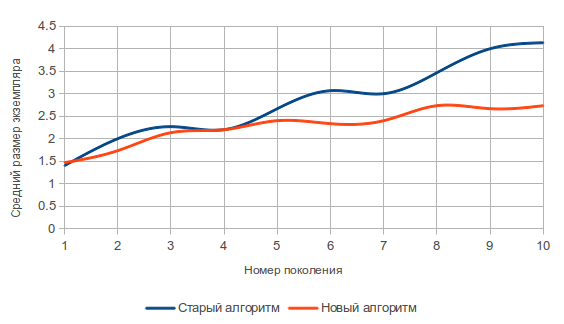
\includegraphics[width=0.6\textwidth]{crossover_difference.png}
  }
\end{figure}
Средняя производная по таким графикам различается в два раза в пользу новой версии алгоритма кроссовера, что говорит о решении данной поставленной задачи по крайней мере в ограниченном объеме.

\section{Модернизация алгоритма мутации}
Для оценки качества модификации алгоритма мутации было проведено равное количество экспериментов при одинаковых начальных условиях для старого и нового алгоритма мутации, для разных вероятностей мутации. Для моделирования старого алгоритма новому задавались нулевыми вероятности мутации всех элементов кроме атомарных - функций ЦОС. Для моделирования аналогичной вероятности с использованием рекурсивной мутации вероятности выставлялись одинаковыми и равными приведенной вероятности рассчитаной по формуле. \ref{equiv_prob}
\begin{equation}
P_{n}=\sqrt[3]{p-1}+1
\label{equiv_prob}
\end{equation}
Где $ p $ - вероятность для плоского случая (приведенная вероятность), а $ P_{n} $ - аналогичная ей вероятность для рекурсивного случая.

На основе экспериментов построены графики \ref{mutate_diff_fit} и \ref{mutate_diff_gen}. На основе графика  \ref{mutate_diff_gen} можно сказать, что после реализации новой версии мутации уменьшилось время сходимости алгоритма, а так как на графике \ref{mutate_diff_fit} видно, что фитнесс-функция оптимального экземпляра не только не ухудшилась но и улучшилась при таком переходе, можно сказать что мы не столкнулись с явлением преждевременной сходимости.
\begin{figure}[H]
 \caption{график средней фитнесс-функции для приведенных вероятностей мутации}\label{mutate_diff_fit}
 \centering{
 	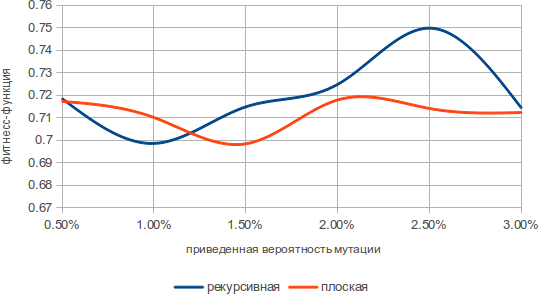
\includegraphics[width=0.6\textwidth]{mutation_difference_fit.png}
  }
\end{figure}
\begin{figure}[H]
 \caption{график поколений сходимости для приведенных вероятностей мутации}\label{mutate_diff_gen}
 \centering{
 	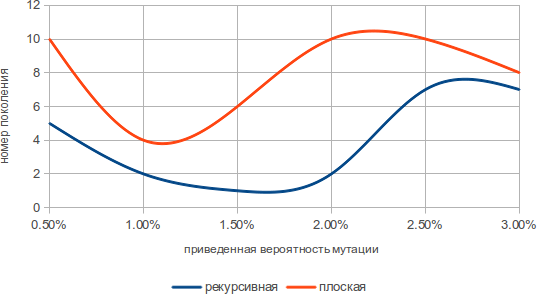
\includegraphics[width=0.6\textwidth]{mutation_difference_gen.png}
  }
\end{figure}



\chapter{Постановка задачи}
В прошлой версии программного обеспечения, реализованного в дипломной работе научного руководителя присутствовала избыточность обучающих данных и слабая сопровождаемость кода.

Основной задачей была реализация новой версии ПО на python с попутным внесением технических и алгоритмических изменений
Основной задачей было избавление от избыточности обучающих данных. В качестве метода решения этой задачи была выбрана модификация алгоритма кроссовера, а точнее смещение вероятности при выборе размера нового экземпляра в сторону уменьшения. В качестве критерия оценки избыточности была выбрана следующая метрика: средний размер экземпляра в популяции \{ на последней итерации || на момент максимума || в течение всех поколений \}

%В качестве средств повышения сопровождаемости кода были выбраны:
%\begin{enumerate}
%\item Смена языка разработки на язык ориентированный на прозрачность исходного кода
%\item Следование рекомендациям PEP8 и PEP257 для разработчиков на языке Python, что приводило код и комментарии к нему к монотипно читаемому виду.
%\item Работа с git в качестве системы контроля версий, что позволяет отследить историю изменений в коде
%\item хранение хода и результатов каждого отдельного эксперимента в виде xml что позволяет провести анализ не только результатов набора экспериментов но и анализ отдельных деталей вплоть до просмотра конкретной хромосомы конкретного экземпляра конкретного поколения в конкретном эксперименте 
%\end{enumerate}

В качестве оценок качества кода и сопровождаемости были выбраны следующие эксперименты, метрики и критерии:
\begin{enumerate}
\item Валидация PEP8 \& PEP257
\item Проведение ряда экспериментов работавших в прошлой версии ПО, как средство проверки правильности практической реализации алгоритма
\item Сравнение характеристик сходимости при старом и новом алгоритме мутации
\end{enumerate}

\chapter{Решение поставленных задач}
В прошлой версии программного обеспечения, реализованного в дипломной работе научного руководителя присутствовал ряд проблем:
\begin{enumerate}
\item Избыточность обучающих данных вызванная алгоритмом кроссовера.
\item Слабая сопровождаемость кода.
\end{enumerate}
\chapter{разнообразная хуита из шаблона.}


В отчётах могут быть и таблицы - см.табл.~\ref{T:T1}.

\begin{longtable}{|c|c|p{110mm}|}
 \multicolumn{3}{l}{\tablename~\thetable~---~Пример таблицы\label{T:T1}}\\\hline
 Название 1  & Название 2 & Название 3 \\
\hline
\endfirsthead
 \multicolumn{3}{l}{Продолжение таблицы~\ref{T:T1}}\\
\hline
1 & 2 & 3 \\
\hline
\endhead
Это  & пример & данных  \\
\hline
помещённых & внутрь & таблицы \\
\hline
\end{longtable}


\backmatter %% Здесь заканчивается нумерованная часть документа и начинаютяс заключение и ссылки

\Conclusion % заключение к отчёту

\begin{thebibliography}{1} %% здесь библиографический список

\bibitem{filosofyNewestdict}
{Грицанов} А.А.~и др.
\newblock {\em Новейший философский словарь}.
\newblock Мн.: Книжный Дом., 2003.

\end{thebibliography}

% \bibliography{biblio/filosofy} %% вместо вставки библиографии можно использовать базы BiBTeX - просто раскомментируйте эту строку.
\end{document}
